\documentclass{acm_proc_article-sp}
\usepackage[utf8]{inputenc}
\usepackage[T1]{fontenc}
\usepackage{graphicx}
\usepackage{epstopdf}
%\usepackage[labelsep=period]{caption}
\usepackage{amssymb,amsmath,mathrsfs}
\usepackage[russian,english]{babel}
\usepackage{array}
%\usepackage{multicol}
\usepackage[ruled,vlined,linesnumbered,algo2e]{algorithm2e}
\usepackage{color}
\usepackage{cmap}
%\usepackage{tikz}
%\usepackage{pgfplots}
%%\usepackage{verbatim}
%\usepackage{standalone}
\usepackage[hyphens]{url}

\tolerance=5000
\hbadness=8000
\newcommand{\const}{\mathrm{const}}
\newcommand{\tsum}{\mathop{\textstyle\sum}\limits}
\newcommand{\tprod}{\mathop{\textstyle\prod}\limits}
\newcommand{\cov}{\mathop{\rm cov}\limits}
\newcommand{\Dir}{\mathop{\rm Dir}\nolimits}
\newcommand{\norm}{\mathop{\rm norm}\limits}
\newcommand{\KL}{\mathop{\rm KL}\nolimits}
%\renewcommand{\geq}{\geqslant}
%\renewcommand{\leq}{\leqslant}
\newcommand{\eps}{\varepsilon}
\newcommand{\cond}{\mspace{3mu}{|}\mspace{3mu}}
\newcommand{\Loss}{\mathscr{L}}
\newcommand{\RR}{\mathbb{R}}
\newcommand{\cL}{\mathscr{L}}
\newcommand{\cP}{\mathscr{P}}
\newcommand{\kw}[1]{\textsf{#1}}
\SetKwFor{ForAll}{\textbf{for all}}{}{}

\newcommand{\vokov}[1]{\textsl{#1}}

\newtheorem{theorem}{Theorem}
\newdef{note}{Note}

%%... and these rows too.
%\pgfplotsset{ every non boxed x axis/.append style={x axis line style=-},
%     every non boxed y axis/.append style={y axis line style=-}}
%\pgfplotsset{compat = 1.3}

\begin{document}
\conferenceinfo{CIKM}{CIKM 2015 Workshop on Topic Models: Post-Processing and Applications}
%\CopyrightYear{2015}
\title{
    Non-Bayesian Additive Regularization for Multimodal~Topic~Modeling of Large Collections
}
\numberofauthors{5}
\author{
    \alignauthor
        Konstantin Vorontsov\\
        \affaddr{Yandex, Moscow Institute of~Physics and Technology}\\
        \email{\footnotesize\sf voron@yandex-team.ru}
    \alignauthor
        Oleksandr Frei\\
        \affaddr{Schlumberger\\ Information Solutions}
        \email{\footnotesize\sf oleksandr.frei@gmail.com}
    \alignauthor
        Anastasia Yanina\\
        \affaddr{Moscow Institute of~Physics and Technology}\\
        \email{\footnotesize\sf yanina.anastasia.mipt@gmail.com}
    \and
    \alignauthor
        Murat Apishev\\
        \affaddr{Moscow State University}\\
        \email{\footnotesize\sf great-mel@yandex.ru}
    \alignauthor
        Peter Romov\\
        \affaddr{Yandex}\\
        \email{\footnotesize\sf peter@romov.ru}
    \alignauthor
        Marina Suvorova\\
        \affaddr{Moscow State University}\\
        \email{\footnotesize\sf m.dudarenko@gmail.com}
}
\date{20 February 2015}
\maketitle

\begin{abstract}
Probabilistic topic modeling of text collections is a powerful tool for statistical text analysis
based on the preferential use of graphical models and Bayesian learning.
Additive regularization for topic modeling (ARTM) is a~recent semi-probabilistic approach, which
provides a~simpler inference for many models previously studied only in the Bayesian settings.
ARTM reduces barriers to entry into topic modeling research field
and facilitates combination of topic models.
%ARTM gives a~natural way to combine regularizers for multi-criteria topic modeling.
In~this paper we develop the multimodal extension of ARTM approach
and implement it in \mbox{BigARTM} open source project %(\texttt{http://bigartm.org})
for online parallelized topic modeling.
We~demonstrate the ability of non-Bayesian regularization
to~combine modalities, languages and multiple criteria
to~find sparse, diverse, and interpretable topics.
\end{abstract}

\keywords{%
    Probabilistic Topic Modeling,
    Probabilistic Latent Sematic Analysis,
    Latent Dirichlet Allocation,
    Additive Regularization of Topic Models,
    Stochastic Matrix Factorization,
    EM-algorithm,
    BigARTM.
}

\section{Introduction}

Topic modeling is a~rapidly developing branch of statistical text analysis~\cite{blei12ptm}.
Topic model reveals a~hidden thematic structure of a~text collection
and finds a~compressed representation of each document in terms of its topics.
Practical applications of topic models include
information retrieval,
%for long-text queries,
%revealing research trends and research fronts,
classification, categorization, summarization and segmentation of texts.
Topic models are increasingly used for non-textual and heterogeneous data
including signals, images, video and networks.
More ideas, models and applications are outlined in the survey~\cite{daud10knowledge}.

From a statistical perspective,
a~probabilistic topic model (PTM)
defines each topic by a~multinomial distribution over words,
and then describes each document with a~multinomial distribution over topics.

Modern literature on topic modeling offers
hundreds of models adapted to different situations~\cite{daud10knowledge}.
Nevertheless,
most of these models are too difficult for practitioners
to quickly understand, adapt and embed into applications.
This leads to a~common practice of tasting only the very basic models such as
\emph{Probabilistic Latent Semantic Analysis}, PLSA~\cite{hofmann99plsi} and
\emph{Latent Dirichlet Allocation}, LDA~\cite{blei03latent}.
Most practical inconveniences are rooted in Bayesian learning,
which is the dominating approach in topic modeling.

Bayesian learning is a very powerful and general theoretical framework,
and topic modeling is just one of its applications.
Bayesian inference is elegant when used with conjugate priors.
However, from the linguistic point of view the Dirichlet conjugate prior
is not necessary the~best choice
as it conflicts with natural assumptions of~sparsity.
Better motivated non-conjugate priors
require a~laborious mathematical work and
lead to intricate learning algorithms.
The development of combined and multi-objective topic models also remains a~challenging task in the Bayesian approach.
An~evolutionary approach to multi-objective Bayesian topic modeling has been proposed in~\cite{khalifa13multi},
but it seems to be computationally infeasible for large text collections.
Until now, there was no freely available software to combine topic models.

From an optimization perspective,
topic modeling can be considered as a~special case
of approximate stochastic matrix factorization.
To~learn a~factorized representation of a~text collection
is an ill-posed problem, which has an infinite set of solutions.
A~typical regularization approach in this case is
to impose problem-specific constraints
in a~form of additive terms in the optimization criterion.

\emph{Additive Regularization of Topic Models} (ARTM)
is a~semi-probabilistic approach based on classical (non-Bayesian) regularization~\cite{voron14dan-eng}.
%ARTM benefits
%from a~more general semi-probabilistic regularization on the one hand and
%from a~more specific stochastic matrix factorization on the other hand.
In~ARTM a~topic model is learned by maximizing a~weighted sum
of the log-likelihood and additional regularization criteria.
These criteria are not required to be log-priors or even to have a~probabilistic sense.
The optimization problem is solved by a~general regularized expectation-maximization (EM) algorithm,
which can be easily applied to any combination of regularization criteria.
The non-Bayesian regularization provides a~much simpler inference
for many topic models previously studied only in the Bayesian setting~\cite{voron14aist,voron14mlj}.
In~particular,
the LDA model can be alternatively understood as a~smoothing regularizer
that minimizes Kullback--Leibler (KL) divergence
of each topic distribution with a~fixed multinomial distribution.
The maximization of the KL-divergence naturally leads to sparsing~\cite{voron14aist}.
This possibility is difficult to see from the Bayesian perspective,
thereby all Bayesian approaches to sparsing are much more complicated~%
\cite{shashanka07sparse,wang09decoupling,ugander11concave,eisenstein11sparse,chien13bayesian}.

ARTM makes topic models easier to design, to explain, to infer, and to combine,
naturally reducing barriers to entry into topic modeling research field.

In~this paper we develop the multimodal extension of ARTM approach
and incorporate its parallel online implementation into BigARTM open source projet.
%In~this paper we develop the ARTM approach in three directions:
%the multiple modalities modeling,
%the online algorithm, and
%the parallel implementation.

Multimodal data has become increasingly important in many application areas.
Large data collections coming from the web or sensor networks
consist of heterogeneous linked data.
Typically, texts are accompanied by images, audio or video clips, usage data,
metadata containing authors, links, date-time stamps, etc.
In~these cases documents are considered as multimodal containers,
where words form the elements of a single modality.
All modalities are useful for determining more relevant topics,
and, vice-versa,
topics are useful for crossmodal retrieval,
making recommendations for users or
making predictions when data of some modalities are missing.
We~introduce the multimodal additively regularized topic model
with an arbitrary number of modalities
and generalize the regularized EM-algorithm for this case.

Online algorithms have proven to be very efficient
for large document collections, including those arriving in a~stream.
Online algorithms are now available for
PLSA~\cite{bassiou14online},
LDA variational inference~\cite{hoffman10online},
LDA stochastic inference~\cite{mimno12sparse}, and
some other topic models.
We~show that the online algorithm is not necessarily associated with
a~particular type of model, nor
a~particular type of inference,
but only with a~certain reorganization of steps in the EM-like iterative process.
Our online algorithm remains the same
for any combination of regularizers and any number of modalities.

The rest of the paper is organized as follows.
%
In~section~\ref{sec:ARTM}
we~introduce notation and definitions of topic modeling and ARTM.
%
In~section~\ref{sec:Multimodal}
we~introduce a~multimodal topic modeling for documents with additional discrete metadata.
%
In~section~\ref{sec:Online}
we~generalize online EM-algorithm from~\cite{hoffman10online} for multimodal ARTM
%
%In~section~\ref{sec:BigARTM}
%we~describe parallel architecture and implementation details of the BigARTM library.
and discuss some details of its parallel implementation in BigARTM library.
%
In~section~\ref{sec:Experiments}
we~report results of our experiments on large datasets.
%%%%BigARTM performs better than Vowpal Wabbit LDA and Gensim libraries
%%%%in terms of perplexity and runtime on Wikipedia corpus.
%%%%Comparing to the other libraries BigARTM offers several additional features,
%%%%such as regularization and multimodality.
%
%In~section~\ref{sec:Conclusions}
%we~conclude with advantages, limitations and open problems.

\section{Additive Regularization for\\ Probabilistic Topic Models}
\label{sec:ARTM}

%Matching Words and Pictures, MoM-LDA \cite{barnard03matching}
%\cite{virtanen12factorized}
%\cite{roller13multimodal}

Let
$D$ denote a finite set (collection) of texts and
$W$ denote a~finite set (vocabulary) of all terms from these texts.
Each term can represent a~single word or a~key phrase.
Each document ${d\in D}$ is a sequence of terms from the vocabulary~$W$.
Assume that
each term occurrence in each document refers to some latent topic from a~finite set of topics~$T$.
Text collection is considered to be a sample of triples
$(w_i,d_i,t_i)$,\; ${i=1,\dots,n}$,
drawn independently from a~discrete distribution $p(w,d,t)$
over the finite probability space $W\times D \times T$.
Terms~$w_i$ and documents~$d_i$ are observable variables,
while topics~$t_i$ are latent variables.

The topic model of Probabilistic Latent Semantic Analysis, PLSA~\cite{hofmann99plsi}
explains the terms probabilities $p(w\cond d)$ in each document~${d\in D}$
by a~mixture of term probabilities for topics and topic probabilities for documents:
\[
    p(w\cond d)
    = \sum_{t\in T} p(w\cond t)\: p(t\cond d)
    = \sum_{t\in T} \phi_{wt} \theta_{td},\;
    w\in W.
\]
This representation follows immediately from the law of total probability
and the assumption of conditional independence $p(w\cond t) = p(w\cond d,t)$,
which means that each topic generates terms regardless of the document.

The parameters
${\theta_{td}=p(t\cond d)}$ and ${\phi_{wt}=p(w\cond t)}$
form matrices
${\Theta = \bigl( \theta_{td} \bigr)_{T\times D}}$ and
${\Phi = \bigl( \phi_{wt} \bigr)_{W\times T}}$.
These matrices are \emph{stochastic},
that~is, their vector-columns represent discrete distributions.
The~number of topics~$|T|$ is usually much smaller than~$|D|$ and~$|W|$.

To learn parameters $\Phi$, $\Theta$ from the collection
we maximize the log-likelihood:
\[
    \cL (\Phi,\Theta) =
    \sum_{d\in D}\sum_{w\in W} n_{dw} \ln p(w\cond d)
    \to \max_{\Phi,\Theta},
\]
where
$n_{dw}$ is the number of occurrences of the term ${w\in W}$ in the document~$d$.

Following the ARTM approach,
we~introduce $r$~additional criteria
$R_i(\Phi,\Theta)$,\; ${i=1,\dots,r}$,
called \emph{regularizers}.
We~would like to maximize them separately,
but the maximization of their linear combination
with nonnegative \emph{regularization coefficients}~$\rho_i$
is technically more convenient:
\[
    R(\Phi,\Theta) =
    \sum_{i=1}^r \rho_i R_i(\Phi,\Theta)
    \;\to\; \max_{\Phi,\Theta}.
\]

Then we add a~regularization term $R(\Phi,\Theta)$ to the log-likelihood
and solve a~constrained multicriteria optimization problem via scalarization:
\begin{gather}
\label{eq:ARTM}
    \cL (\Phi,\Theta) + R(\Phi,\Theta) \to \max_{\Phi,\Theta};
\\\label{eq:ARTM:norm}
    \sum_{w\in W}\!\!\! \phi_{wt} = 1,~
    \phi_{wt}\geq 0;
    \qquad
    \sum_{t\in T} \theta_{td} = 1,~
    \theta_{td}\geq 0.
\end{gather}

It follows from Karush--Kuhn--Tucker conditions
that the \mbox{local} maximum $(\Phi,\Theta)$
of the problem~\eqref{eq:ARTM},~\eqref{eq:ARTM:norm}
satisfies the following system of equations
with auxiliary variables interpreted as conditional probabilities
${p_{tdw} = p(t\cond d,w)}$~\cite{voron14aist}:
\begin{align}
    \label{eq:ARTM:Estep}
    p_{tdw} &= \norm_{t\in T} \bigl(\phi_{wt}\theta_{td}\bigr);
\\
    \label{eq:ARTM:Mstep:phi}
    n_{wt} &= \sum_{d\in D} n_{dw} p_{tdw};\quad
    \phi_{wt} = \norm_{w\in W}
        \biggl(
            n_{wt} + \phi_{wt} \frac{\partial R}{\partial \phi_{wt}}
        \biggr);
\\
    \label{eq:ARTM:Mstep:theta}
    n_{td} &= \sum_{w\in d} n_{dw} p_{tdw};\quad
    \theta_{td} = \norm_{t\in T}
        \biggl(
            n_{td} + \theta_{td} \frac{\partial R}{\partial \theta_{td}}
        \biggr);
\end{align}
where the ``norm'' operator transforms
a~real vector $(x_t)_{t\in T}$ to
a~vector $(\tilde x_t)_{t\in T}$ with a discrete distribution:
\[
    \tilde x_t = \norm_{t\in T} x_t = \frac{\max\{x_t,0\}}{\sum\limits_{s\in T} \max\{x_s,0\}}.
\]
The system \eqref{eq:ARTM:Estep}--\eqref{eq:ARTM:Mstep:theta}
can be~solved by various numerical methods,
for example by the simple-iteration method,
or, equivalently, by the EM-algorithm.
%Both methods are commonly used in~practice.

Many Bayesian topic models can be considered
as special cases of ARTM with different regularizers~\cite{voron14aist,voron14mlj}.
For~example,
PLSA~\cite{hofmann99plsi} corresponds to the absence of regularization, ${R=0}$.
LDA~\cite{blei03latent} corresponds to the smoothing regularizer,
which minimizes the KL-divergences
$KL(\alpha\|\theta_d)$ and
$KL(\beta\|\phi_t)$
for fixed distributions $\beta$, $\alpha$.
Choosing uniform distributions for $\beta$ and $\alpha$
corresponds to symmetric Dirichlet priors in Bayesian approach.

Additivity of ARTM models let users build topic models for various applications
simply by choosing a~suitable combination of~predefined regularizers
from an extendable \mbox{library}.
%
For~example,
in \cite{voron14mlj} as many as five regularizers are combined together to improve interpretability of the model.
The key idea is to split the set of topics $T$ into two subsets: ${T = S \sqcup B}$,
and to configure regularizers in such a way that
domain-specific terms go into the set $S$,
while commonly used words land in the set $B$.
Sparsity of \emph{domain topics} $t \in S$ is promoted by a regularizer that maximize the KL-divergences
$KL(\alpha\|\theta_d)$ and
$KL(\beta\|\phi_t)$.
Smoothness of \emph{background topics} $t \in B$ is promoted by minimizing KL-divergences
$KL(\alpha\|\theta_d)$ and
$KL(\beta\|\phi_t)$.
Finally, a covariance regularizer is used to
decrease the correlation between columns in the $\Phi$~matrix, thus promoting the diversity of the topics.
The final combination of regularizers is as follows:
\begin{align*}
    R(\Phi,\Theta)
    =&
    - \beta_0 \sum_{t\in S} \sum_{w\in W} \beta_w \ln \phi_{wt}
    - \alpha_0 \sum_{d\in D} \sum_{t\in S} \alpha_t \ln \theta_{td}
    \notag
\\  {}&
    + \beta_1 \sum_{t\in B} \sum_{w\in W} \beta_w \ln \phi_{wt}
    + \alpha_1 \sum_{d\in D} \sum_{t\in B} \alpha_t \ln \theta_{td}
\\  {}&
    - \gamma
        \sum_{t\in T}
        \sum_{s\in T\backslash t}
        \sum_{w\in W} \phi_{wt}\phi_{ws},
\end{align*}
where $\beta_0$, $\alpha_0$, $\beta_1$, $\alpha_1$, $\gamma$
are regularization coefficients.

This combination was extended in~\cite{voron14aist} by a new regularizer that maximizes the KL-divergence
$KL\bigl( \frac1{|T|}\|p(t) \bigr)$,
leading to a topic selection.
Starting from an excessively high number of topics
the regularizer eliminates insignificant, duplicated, and linearly dependent topics~\cite{voron15slds}.
Compared to Hierarchical Dirichlet Process~\cite{teh06hierarchical}, the new regularizer results in a better topic selection algorithm:
it gives a~more stable number of~topics, takes less time to execute,
and has an ability to combine it with other topic models via additive regularization.

An important subject for ARTM models is optimization of the regularization coefficients~$\rho_i$.
According to Tikhonov's theory of~ill-posed inverse problems~\cite{tihonov77methods-eng},
the regularization coefficients must tend to zero with the number of iteration.
%In~this case we can achieve a~stable solution.
In~practice,
the regularization path is selected
by~adaptive tuning of regularization coefficients~\cite{voron14mlj,voron14aist,voron15slds}.
This empirical technique is based on visual control of
multiple intrinsic and extrinsic performance measures
on each iteration.

\section{Multimodal ARTM}
\label{sec:Multimodal}

%Matching Words and Pictures, MoM-LDA \cite{barnard03matching}
%\cite{virtanen12factorized}
%\cite{roller13multimodal}

Now assume that
a~document can contain not only words, but also terms of other modalities.
Each modality is defined by a finite set (vocabulary) of terms $W^m$, ${m=1,\dots,M}$.
The sets $W^m$ are disjoint.

Examples of not-word modalities are:
authors,
class or category labels,
date-time stamps,
references to/from other documents/authors,
named entities,
objects found in the images associated with the documents,
users that read or downloaded documents,
advertising banners,
etc.

As in the previous section,
the collection is considered to be a sample of i.i.d. triples
$(w_i,d_i,t_i) \sim p(w,d,t)$
drawn from the finite probability space $W\times D \times T$,
but now ${W=W^1\sqcup\cdots\sqcup W^M}$
is a~disjoint union of the vocabularies across all modalities.

Following the idea of Correspondence LDA~\cite{blei03modeling}
and Dependency LDA~\cite{rubin12statistical}
we introduce a topic model $p(w\cond d)$
for each modality $W^m$,\; $m=1,\dots,M$:
\[
    p(w\cond d)
    = \sum_{t\in T} p(w\cond t)\: p(t\cond d)
    = \sum_{t\in T} \phi_{wt} \theta_{td},\;
    w\in W^m.
\]
Stochastic matrices ${\Phi^m = \bigl( \phi_{wt} \bigr)_{W^m\times T}}$
of \emph{term probabilities for the topics},
if stacked vertically, form a~${W\!\!\times\!T}$-matrix~$\Phi$.

To learn parameters $\Phi^m$, $\Theta$ from the multimodal collection
we maximize the log-likelihood for each $m$-th modality:
\[
    \cL_m (\Phi^m,\Theta) =
    \sum_{d\in D}\sum_{w\in W^m} n_{dw} \ln p(w\cond d)
    \to \max_{\Phi^m,\Theta},
\]
where
$n_{dw}$ is the number of occurrences of the term ${w\in W^m}$ in the document~$d$.
Note that topic distributions of documents $\Theta$ are common for all modalities.

In ARTM we add a~weighted sum of regularization criteria $R(\Phi,\Theta)$ to the log-likelihood
and solve a~constrained multicriteria optimization problem:
\begin{gather}
\label{eq:multimodal}
    \sum_{m=1}^M \tau_m \cL_m (\Phi^m,\Theta)
    + R(\Phi,\Theta)
    \to \max_{\Phi,\Theta};
\\\label{eq:multimodal:norm}
    \sum_{w\in W^m}\!\!\! \phi_{wt} = 1,~
    \phi_{wt}\geq 0;
    \qquad
    \sum_{t\in T} \theta_{td} = 1,~
    \theta_{td}\geq 0;
\end{gather}
where \emph{regularization coefficients}~$\tau_m$
are used to~balance the importance of different modalities.
The local maximum $(\Phi,\Theta)$
of the problem~\eqref{eq:multimodal},~\eqref{eq:multimodal:norm}
satisfies the following system of equations
with auxiliary variables $p_{tdw} = p(t\cond d,w)$:
\begin{align}
    \label{eq:Estep}
    p_{tdw} &= \norm_{t\in T} \bigl(\phi_{wt}\theta_{td}\bigr);
\\\notag
    n_{wt} &= \sum_{d\in D} \tau_{m(w)} n_{dw} p_{tdw};
\\\notag
    n_{td} &= \sum_{w\in d} \tau_{m(w)} n_{dw} p_{tdw};
        %\sum_{m=1}^M \tau_m \!\!\sum_{w\in W^m}\!\!\! n_{dw} p_{tdw};
\\
    \label{eq:Mstep:phi}
    \phi_{wt} &= \norm_{w\in W^m}
        \biggl(
            n_{wt} + \phi_{wt} \frac{\partial R}{\partial \phi_{wt}}
        \biggr);
\\
    \label{eq:Mstep:theta}
    \theta_{td} &= \norm_{t\in T}
        \biggl(
            n_{td} + \theta_{td} \frac{\partial R}{\partial \theta_{td}}
        \biggr);
\end{align}
where $m(w)$~is the modality of the term~$w$,\; $w\in W^{m(w)}$.

The system of equations \eqref{eq:Estep}--\eqref{eq:Mstep:theta}
follows from Karush--Kuhn--Tucker conditions (see Appendix~A for the proof).
For single modality (${M=1}$) it gives the regularized EM algorithm
described in the previous section.
%%%proposed in~\cite{voron14dan-eng}.

Many previous topic models for labeled documents
can be considered as specials cases of multimodal ARTM.
Most of them are based on LDA model and use Dirichlet priors,
which correspond to smoothing regularization.
From ARTM perspective,
there is little reason to always use only the smoothing regularizer.

The following topic models exactly correspond to the multimodal ARTM,
up~to the modality sense.
A~topic model of document content and hypertext connectivity~\cite{cohn00missing}
introduces a modality to represent hyperlinks between documents.
The Conditionally Independent LDA, CI-LDA~\cite{newman06entity}
has the modality of named entities mentioned in a~given document.
The Tag-LDA \cite{si09taglda}
has the modality of tags as a special kind of words.
The LDA-JS and LDA-post~\cite{dietz07unsupervised}
has the modality of publications cited in a~given document;
an additional regularizer takes into account that cited documents are likely to share similar topics.
Both models are designed to estimate the strength of influence of cited publications.
The Dependency LDA~\cite{rubin12statistical}
has the modality of document categories or class labels.
The MultiLingual LDA, ML-LDA~\cite{ni09mining} and
the PolyLingual Topic Model, PLTM~\cite{mimno09polylingual}
have $L$~modalities for $L$~different languages;
parallel documents always share one identical topic distribution.
The BiLingual LDA, BiLDA~\cite{smet09weblinking}
is also a~multilanguage topic model, but the number of modalities is restricted to two.


\section{Online parallel EM-algorithm}
\label{sec:Online}
%\cite{zhang13sparse}

Like Online LDA \cite{hoffman10online} and Online PLSA \cite{bassiou14online}
we split the collection~$D$ into batches~$D_b$, ${b=1,\dots,B}$,
and organize EM iterations so that
each document vector $\theta_d$ is~iterated until convergence at a~constant matrix~$\Phi$,
see Algorithm~\ref{alg:Online} and~\ref{alg:ProcessBatch}.
The matrix~$\Phi$ is updated rarely, after all documents from the batch are processed.
For a~large collection
the matrix~$\Phi$ often stabilizes after small initial part of the collection is processed.
Therefore a~single pass through the collection might be sufficient to learn a~topic model.
The second pass may be needed for the initial part of the collection.

The online reorganization of the EM iterations
is not necessarily associated with Bayesian inference used in~\cite{hoffman10online}.
Different topic models, from PLSA to multimodal and regularized models,
can be learned by the above online EM algorithm.

Algorithm~\ref{alg:Online} does not specify how often to synchronize the~matrix~$\Phi$
at steps~\ref{alg:sync-begin}--\ref{alg:sync-end}.
It~can be done after every batch or less frequently
(for instance if $\frac{\partial R}{\partial \phi_{wt}}$ takes long time to evaluate).
This flexibility is important for concurrent implementation of the algorithm,
where multiple batches are processed in parallel.
In~this case synchronization can be triggered when a fixed number of documents had been processed since the last synchronization.

%\section{BigARTM architecture}
%\label{sec:BigARTM}
%\nopagebreak
%The main goal for BigARTM architecture is to ensure a constant memory usage regardless of the collection size.
%For this reason

Each $D_b$ batch is stored on disk in a separate file,
and only a limited number of batches is loaded into the main memory at any given time.
The entire $\Theta$ matrix is also never stored in the memory.
As a result, the memory usage stays constant regardless of the size of the collection.

%%\paragraph{Concurrency}
%%A~general rule of concurrency design is
%To express parallelism at the highest possible level
%%For this reason BigARTM
%we implement a concurrent processing of the batches
%and keep a~single-threaded code for the $\kw{ProcessBatch}(D_b, \phi_{wt})$ routine.

To split collection into batches and process them concurrently is a common approach,
introduced in AD-LDA algorithm \cite{newman09distributed}, and
then further developed in PLDA \cite{wang09plda} and PLDA{+} \cite{liu11plda} algorithms.
These algorithms require all concurrent workers to become idle before an update of the $\Phi$ matrix.
Such synchronization step adds a large overhead in the online algorithm where $\Phi$ matrix is updated multiple times on each iteration.
An alternative architecture without the synchronization step is described in \cite{smola10architecture},
however it mostly targets a distributed cluster environment.
In our work we develop an efficient single-node architecture where all workers benefit from the shared memory space.

\SetAlgoSkip{}
\begin{algorithm2e}[t]
\caption{Online EM-algorithm for multimodal ARTM}
\label{alg:Online}
\BlankLine
\KwIn{collection $D_b$, discounting factor $\rho\in(0,1]$;}
\KwOut{matrix $\Phi$;}
\BlankLine
initialize $\phi_{wt}$ for all $w \in W$ and $t \in T$\;
$n_{wt} := 0$,~ $\tilde n_{wt} := 0$ for all $w \in W$ and $t \in T$\;
\ForAll{batches $D_b$, $b = 1,\dots,B$}{
    $(\tilde n_{wt}) := (\tilde n_{wt}) + \kw{ProcessBatch}(D_b, \Phi)$\;
    \If{(synchronize)\label{alg:sync-begin}}{
        $n_{wt} := \rho n_{wt} + \tilde n_{dw}$ for all $w \in W$ and $t \in T$\; \label{alg:merging}
        $\phi_{wt} := \norm_{w\in W^m}
            \bigl(
                n_{wt} + \phi_{wt} \frac{\partial R}{\partial \phi_{wt}}
            \bigr)$
        for all $w \in W^m$,\, $m=1,\dots,M$ and $t \in T$\; \label{alg:phi}

        $\tilde n_{wt} := 0$ for all $w \in W$ and $t \in T$\; \label{alg:sync-end}
    }
}
\end{algorithm2e}

\begin{algorithm2e}[t]
\caption{\kw{ProcessBatch}($D_b, \Phi$)}
\label{alg:ProcessBatch}
\BlankLine
\KwIn{batch $D_b$, matrix $\Phi=(\phi_{wt})$;}
\KwOut{matrix $(\tilde n_{wt})$;}
\BlankLine
$\tilde n_{wt} := 0$ for all $w \in W$ and $t \in T$\;
\ForAll{$d \in D_b$}{
	initialize $\theta_{td} := \frac{1}{|T|}$ for all $t \in T$\;
	\Repeat{$\theta_d$ converges}{
        $p_{tdw} := \norm_{t\in T} \bigl(\phi_{wt}\theta_{td}\bigr)$ for all $w\in d$ and $t \in T$\;
        $n_{td} := \sum_{w\in d} \tau_{m(w)} n_{dw} p_{tdw}$ for all $t \in T$\;
        $\theta_{td} := \norm_{t\in T}
            \bigl(
                n_{td} + \theta_{td} \frac{\partial R}{\partial \theta_{td}}
            \bigr)$ for all $t \in T$\;
	}
	$\tilde n_{wt} := \tilde n_{wt} + \tau_{m(w)} n_{dw} p_{tdw}$ for all $w \in d$ and $t \in T$\;
}
\end{algorithm2e}

\begin{figure}[t]
\begin{centering}
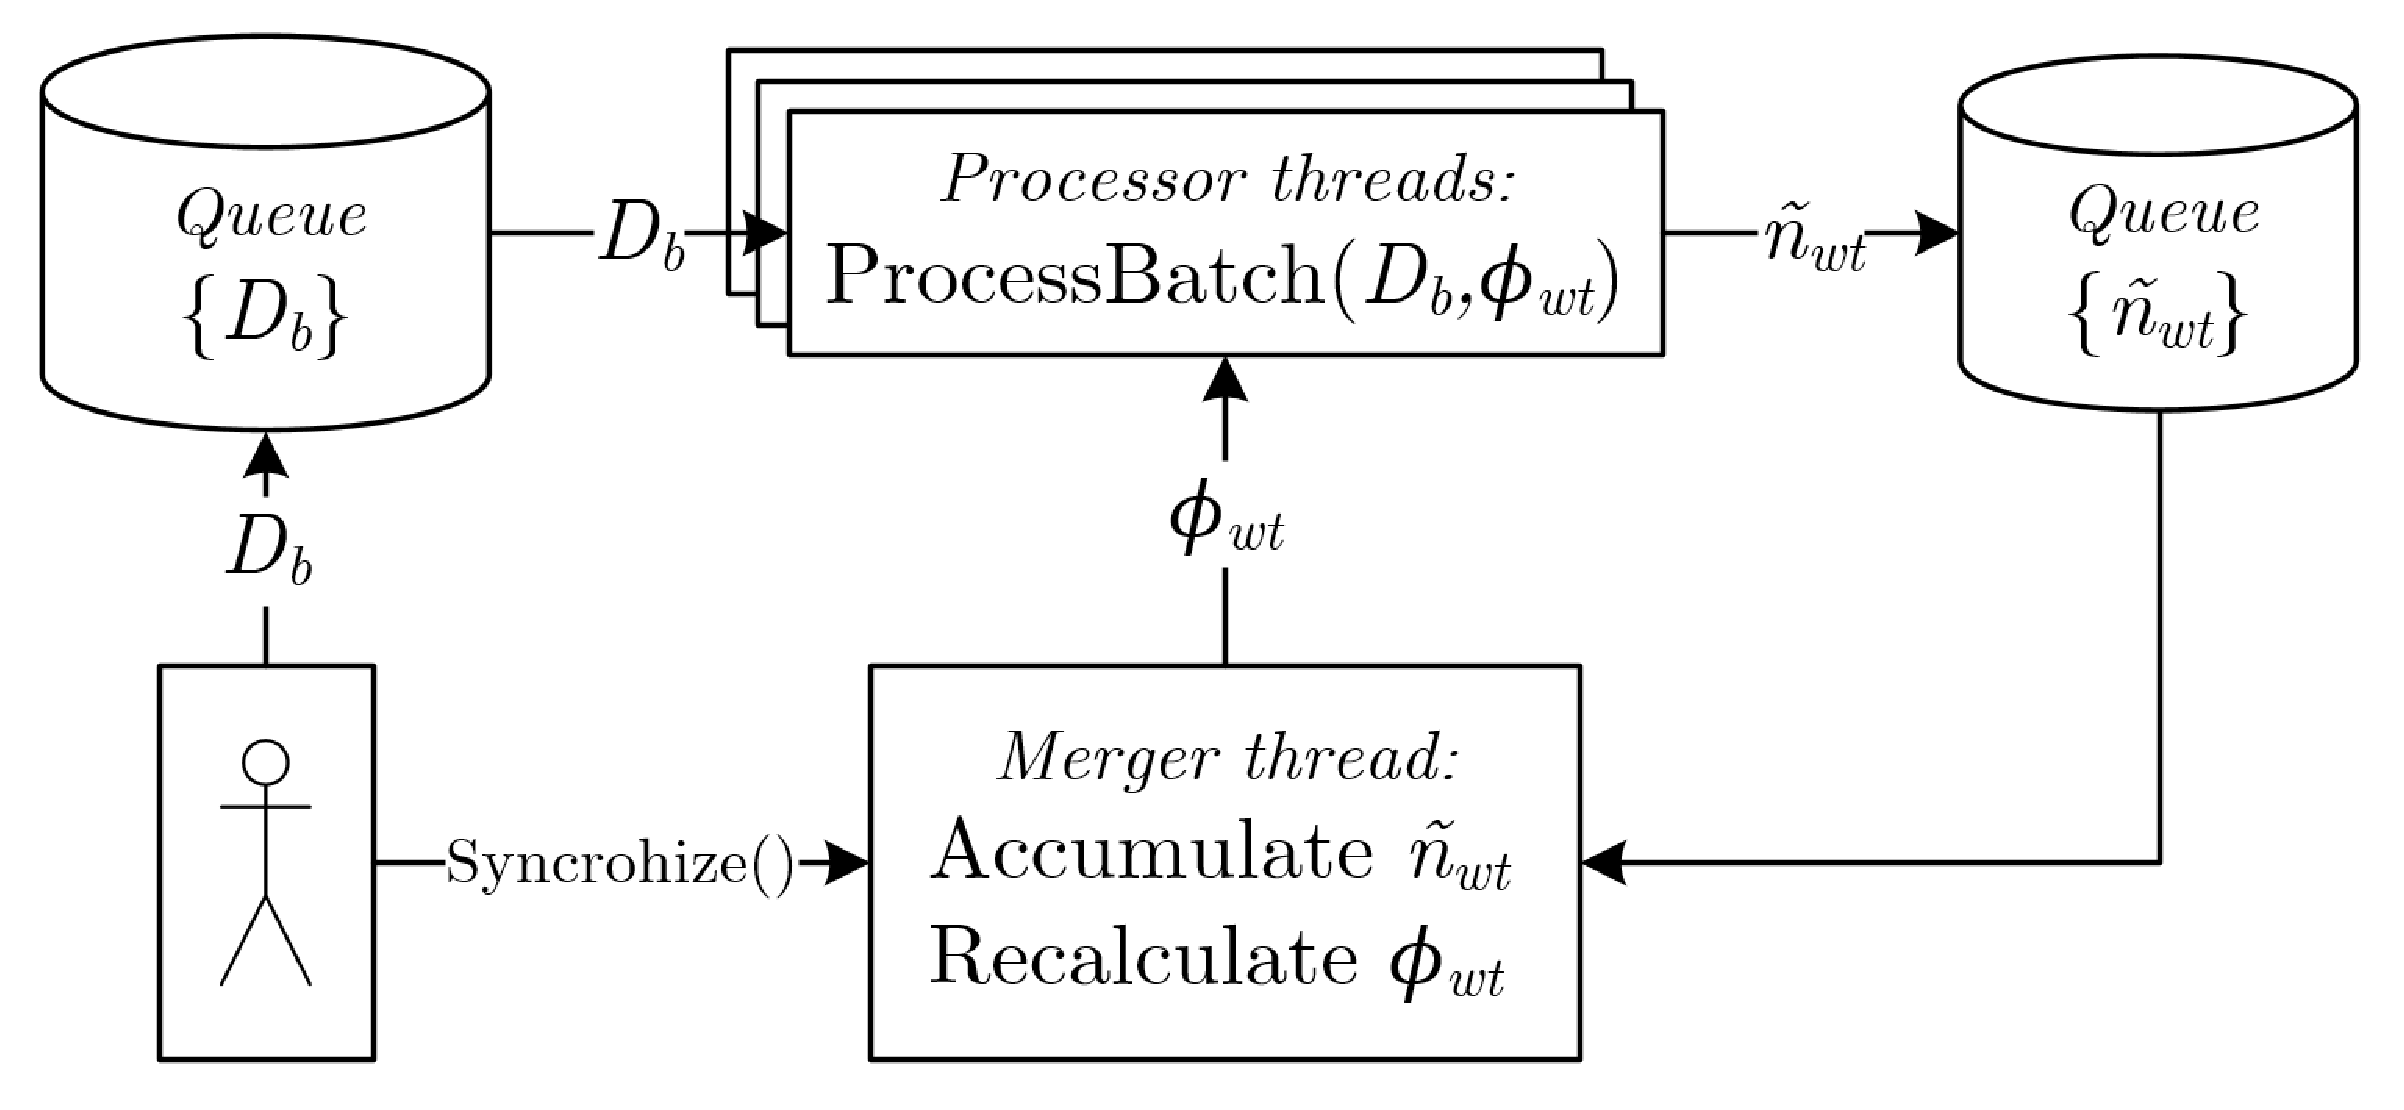
\includegraphics[height=36mm]{diagramm_artm_core.eps}
\caption{Diagram of parallelization components}
\label{fig:diagramm_artm_core}
\end{centering}
\end{figure}

To run multiple $\kw{ProcessBatch}$ in parallel the inputs and outputs of this routine are stored in two separate in-memory queues,
locked for push and pop operations with spin locks.
This approach does not add any noticeable synchronization overhead because
both queues only store smart pointers to the actual data objects,
so push and pop operations does not involve copying or relocating objects in the memory.

Smart pointers are also essential for lifecycle of the $\Phi$ matrix.
This matrix is \emph{read} by all processors threads, and can be \emph{written} at any time by the merger thread.
To update $\Phi$ without pausing all processor threads we keep two copies~--- an \emph{active $\Phi$} and a \emph{background $\Phi$} matrices.
The active matrix is read-only, and is used by the processor threads.
The background matrix is being built in a background by the merger thread
at steps \ref{alg:merging} and~\ref{alg:phi} of Algorithm~\ref{alg:Online},
and once it is ready merger thread marks it as active.
Before processing a new batch the processor thread gets the current active matrix from the merger thread.
This object is passed via shared smart pointer to ensure that processor thread can keep ownership of its $\Phi$ matrix
until the batch is fully processed.
As a result, all processor threads keep running concurrently with the update of $\Phi$ matrix.

All processor threads share the same $\Phi$ matrix,
which means that memory usage stays at constant level regardless of how many cores are used for computation.
Using memory for two copies of the $\Phi$ matrix in our opinion gives a reasonable usage balance between memory and CPU resources.
An~alternative solution with only one $\Phi$ matrix is also possible, but it would require a heavy usage of atomic CPU instructions.
Such operations are very efficient, but still come at a considerable synchronization cost,%
\footnote{\url{http://stackoverflow.com/questions/2538070/atomic-operation-cost}}
and using them for all reads and writes of the $\Phi$ matrix would cause a significant performance degradation for merger and processor threads.
Besides, an arbitrary overlap between reads and writes of the $\Phi$ matrix eliminates any possibility of producing a deterministic result.
The design with two copies of the $\Phi$ matrix gives much more control over this
and in certain cases allows the algorithm to behave in a fully deterministic way.

The design with two $\Phi$ matrices only supports a~single merger thread,
and we believe it should handle all $\tilde n_{wt}$ updates coming from many threads.
This is a reasonable assumption because
merging at step~\ref{alg:merging} takes only about $O(|W|\cdot|T|)$ operations to execute, while
$\kw{ProcessBatch}$ takes $O(n |T| I)$ operations,
where
$n$~is the number of non-zero entries in the batch,
$I$~is the average number of inner iterations in $\kw{ProcessBatch}$ routine.
The ratio $n / |W|$ is typically from 100 to 1000 (based on datasets in UCI Bag-Of-Words repository),
and $I$ is $10 \dots 20$, so the ratio safely exceeds the expected number of cores
(up to 32 physical CPU cores in modern workstations, and even 60 cores of the Intel Xeon Phi co-processors).

%\paragraph{Data layout}
%BigARTM uses
We use dense single-precision matrices to represent $\Phi$ and~$\Theta$.
Together with the $\Phi$ matrix we store a global dictionary of all terms ${w \in W}$.
This dictionary is implemented as $\kw{std::unordered\_map}$ that maps a string representation of ${w \in W}$
into its integer index in the $\Phi$ matrix.
This dictionary can be extended automatically as more and more batches came through the system.
To achieve this each batch $D_b$ contains a local dictionary $W_b$, listing all terms that occur in the batch.
The $n_{dw}$ elements of the batch are stored as a~sparse CSR matrix (Compressed Sparse Raw format),
where each row correspond to a~document ${d \in D_b}$,
and terms~$w$ run over a~local batch dictionary~$W_b$.

For performance reasons $\Phi$ matrix is stored in column-major order, and $\Theta$ in row-major order.
This layout ensures that $\sum_t \phi_{wt} \theta_{td}$ sum runs on contiguous memory blocks.
In both matrices all values smaller than $10^{-16}$ are always replaced with zero to avoid performance issues with denormalized numbers.%
\footnote{\url{http://en.wikipedia.org/wiki/Denormal_number#Performance_issues}}
%http://stackoverflow.com/questions/9314534/why-does-changing-0-1f-to-0-slow-down-performance-by-10x

The parallel online EM-algorithm for multimodal ARTM is implemented in
BigARTM open source project available from \texttt{http://bigartm.org}
under the New BSD License.
The~core of the library is written in C++ and is exposed via two equally rich APIs for C++ and Python.
The~library is cross-platform and can be built for Linux, Windows and OS X in both 32 and 64 bit configuration.

%\paragraph{Programming interface}
%All functionality of BigARTM is expressed in a set of $\kw{extern C}$ methods.
%To input and output complex data structures the API uses Google Protocol Buffers%
%\footnote{\url{http://code.google.com/p/protobuf/}}.
%This approach makes it easy to integrate BigARTM into any research or production environment,
%as almost every modern language has an implementation of Google Protocol Buffers
%and a way of calling $\kw{extern C}$ code
%($\kw{ctypes}$ module for Python, $\kw{loadlibrary}$ for Matlab, $\kw{PInvoke}$ for C\#, etc).
%
%On top of the $\kw{extern C}$ API BigARTM already has convenient wrappers in C++ and Python.
%We are also planning to implement a Java wrapper in the near future.
%In addition to the APIs the library also has a simple CLI interface.
%
%BigARTM has built-in libraries of regularizers and quality measures
%that can be extended in current implementation only through project recompilation.
%
%\paragraph{Basic tools}
%A careful selection of the programming tools is important for any software project.
%This is especially true for BigARTM as its code is written in C++,
%a language that by itself offers less functionality comparing to Python, .NET Framework or Java.
%To mitigate this we use
%various parts of the Boost C++ Libraries,
%Google Protocol Buffers for data serialization,
%ZeroMQ library for network communication,
%and several other libraries.
%%This tools are not specific for topic modeling, and should be considered for any scientific library written in C++.
%
%BigARTM uses CMake as a cross-platform build system,
%and it successfully builds on Windows, Linux and OS X in 32 and 64 bit configurations.
%Building the library require a recent C++ compiler with C++11 support (GNU GCC 4.6.3, clang 3.4 or Visual Studio 2012 or newer),
%and Boost Libraries 1.46.1 or newer. All the other third-parties are included in BigARTM repository.
%
%We also use free online services
%to store source code (\url{https://github.com}),
%to host online documentation (\url{https://readthedocs.org}) and
%to run automated continuous integration builds (\url{http://travis-ci.org}).

\section{Experiments}
\label{sec:Experiments}

\paragraph{Runtime performance}
In first experiment we evaluate the runtime performance and intrinsic quality of BigARTM
against two popular software packages~---
Gensim~\cite{rehurek10software}
%\footnote{\url{http://radimrehurek.com/gensim/}}
and Vowpal Wabbit.%
\footnote{\url{https://github.com/JohnLangford/vowpal_wabbit/}}

All three libraries (VW.LDA, Gensim and BigARTM) work out-of-core,
e.\,g. they are designed to process data that is too large to fit into a computer's main memory at one time.
This allowed us to benchmark on a fairly large collection --- 3.7 million articles from the English Wikipedia.%
\footnote{\url{http://dumps.wikimedia.org/enwiki/20141208/}}
The conversion to bag-of-words was done with $\kw{gensim.make\_wikicorpus}$ script,%
\footnote{\url{https://github.com/piskvorky/gensim/tree/develop/gensim/scripts/}}
which excludes all non-article pages (such as category, file, template, user pages, etc),
and also pages that contain less than $50$~words.
The dictionary is formed by all words that occur in at least 20~documents,
but no more than in $10\%$ documents in the collection.
The resulting dictionary was caped at $|W| = 100\,000$ most frequent words.
Perplexity is used as an intrinsic quality measure:
\begin{equation}
    \label{eq:perplexity}
    \mathscr{P}(D, p) =
        %\exp\left(- \frac{1}{n} L(\Phi, \Theta) \right) =
        \exp \biggl( - \frac{1}{n} \sum_{d \in D} \sum_{w \in d} n_{dw} \ln p(w \cond d) \biggr).
\end{equation}

%There is no article to quote for VW, check http://www.research.rutgers.edu/~lihong/pub/Qin13Efficient.pdf - they use a footnote to quote VW
\emph{Vowpal Wabbit (VW)} is a library
of online algorithms that cover a wide range of machine learning problems. %, not specifically limited to topic modeling.
For~topic modeling VW has the VW.LDA algorithm, based on the Online Variational Bayes LDA \cite{hoffman10online}.
VW.LDA is neither multi-core nor distributed,
but an effective single-threaded implementation in C++ made it one of the fastest tools for topic modeling.% within single computing node.

\emph{Gensim} library specifically targets the area of topic modeling and matrix factorization.
It has two LDA implementations --- LdaModel and LdaMulticore,
both based on the same algorithm as VW.LDA (Online Variational Bayes LDA~\cite{hoffman10online}).
Gensim is entirely written in Python. Its high performance is achieved through the usage of NumPy library,
built over low-level BLAS libraries (such as Intel MKL, ATLAS, or OpenBLAS).
In~LdaModel all batches are processed sequentially, and the concurrency happens entirely within NumPy. % (in numpy.dot, numpy.sum and other Level1 BLAS operations).
In~LdaMulticore the workflow is similar to \mbox{BigARTM} --- several batches are processed concurrently,
and there is a single aggregation thread that asynchronously merges the results.

\begin{table}[t]
	\caption{
        The comparison of BigARTM with VW.LDA and Gensim;
        \emph{train} is the time for model training,
        \emph{inference} is the time for calculation of $\theta_d$ of $100\,000$ held-out documents,
        \emph{perplexity} is calculated according to \eqref{eq:perplexity} on held-out documents.
    }
	\label{tab:libraries_comparison}
    \centering\tabcolsep=4.3pt
	\begin{tabular}[t]{l|c|rrr}
	\hline
	library & procs & train & inference & perplexity \\
	\hline
	BigARTM & 1 & 35 min & 72 sec & 4000 \\
	LdaModel & 1 & 369 min & 395 sec & 4161  \\
	VW.LDA & 1 & 73 min & 120 sec & 4108 \\
	\hline
	BigARTM & 4 & 9 min & 20 sec & 4061  \\
	LdaMulticore & 4 & 60 min & 222 sec & 4111  \\	
	\hline
	BigARTM & 8 & 4.5 min & 14 sec & 4304  \\
	LdaMulticore & 8 & 57 min & 224 sec & 4455 \\
	\hline
	\end{tabular}
\end{table}
%
%\begin{figure}[t]
%	\centering
%	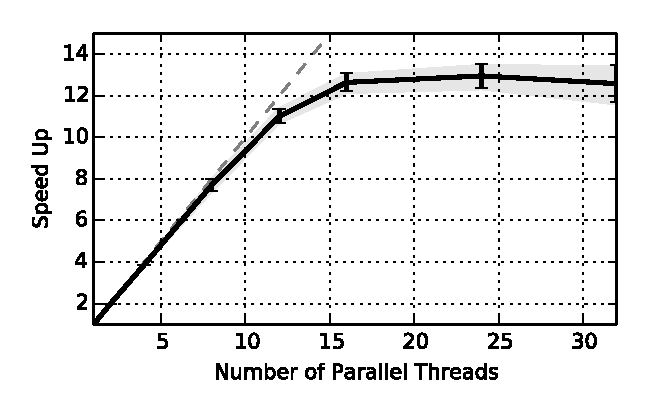
\includegraphics[height=35mm]{bigartm_speedup.eps}
%	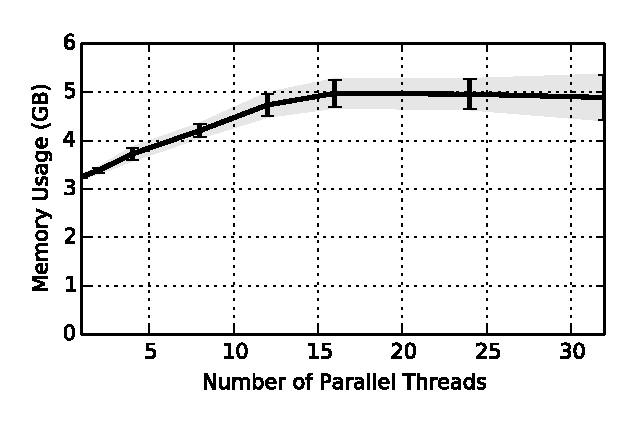
\includegraphics[height=35mm]{bigartm_memory.eps}
%	\caption{Running BigARTM in parallel: speed up (upper chart) and memory usage (lower chart)}
%	\label{fig:bigartm_speedup}
%\end{figure}

Table\;\ref{tab:libraries_comparison} compares the performance of
VW.LDA, Gensim LdaModel and LdaMulticore (\mbox{v0.10.3} under Python~\mbox{2.7}), and BigARTM,
using Amazon EC2 c3.8xlarge instance (Intel-based CPU with 16~physical cores and hyper-threading).
%
Each run performs one pass over the Wikipedia corpus and produces a~model with $|T|=100$ topics.
The collection was split into batches with $10$K documents each
(\texttt{chunksize} in Gensim, \texttt{minibatch} in VW.LDA).
The update rule in online algorithm used a discounting factor
${\rho = (b + \tau_0)^{-0.5}}$,
where $b$ is the number of batches processed so far,
and $\tau_0$ is a~constant offset parameter introduced in~\cite{hoffman10online},
in~our experiment ${\tau_0 = 64}$.
\mbox{Updates} were performed after each batch in non-parallel runs, and after $P$ batches when running in $P$ threads.
To~make a fair comparison we have configured BigARTM to only use the smoothing regularizers, which is~equivalent to the LDA model.
LDA priors were fixed as ${\alpha = 0.1}$,\, ${\beta = 0.1}$ for all models.

\paragraph{Combination of regularizers}

All regularizers built-in \mbox{BigARTM} library can be used in any combination.
In~the following experiment we combine regularizers described in~section~\ref{sec:ARTM}:
sparsing of~$\phi_{t}$, sparsing of~$\theta_{d}$, and pairwise decorrelation of~$\phi_{t}$ distributions.
This combination improves several quality measures without significant loss of perplexity
for the offline implementation of ARTM~\cite{voron14aist}.
The goal of our experiment is to show that the same remains true
for the online implementation in BigARTM.
We~use the following built-in performance measures:
the hold-out perplexity,
the sparsity of $\Phi$ and $\Theta$ matrices, and
several characteristics (size, purity, and contrast) of the topic's lexical kernels, averaged across all topics.
%
Table \ref{tab:model_comparison} compares the results of additive combination of regularizers (ARTM) and the usual LDA model.
Figure~\ref{fig:comparison_plot} presents performance measures as functions of the number of processed documents.
The first chart shows perplexity and sparsity of $\Phi$, $\Theta$ matrices, and
the second chart shows average lexical kernel measures.

\begin{table}[t]
    \caption{Comparison of LDA and BigARTM models:
        $\mathcal{P}_{10k}$, $\mathcal{P}_{100k}$ --- hold-out perplexity on 10K and 100K documents sets,
        $\mathcal{S}_{\Phi}$, $\mathcal{S}_{\Theta}$ --- sparsity of $\Phi$ and $\Theta$ matrices (in \%),
        $\mathcal{K}_{s}$, $\mathcal{K}_{p}$, $\mathcal{K}_{c}$ --- average topic kernel size, purity and contrast respectively.}
    \label{tab:model_comparison}
    \centering\tabcolsep=4.6pt
    \begin{tabular}[t]{l|rrrrrrr}
    \hline
    Model & $\mathcal{P}_{10k}$ & $\mathcal{P}_{100k}$ &  $\mathcal{S}_{\Phi}$ & $\mathcal{S}_{\Theta}$ &  $\mathcal{K}_{s}$ & $\mathcal{K}_{p}$ &  $\mathcal{K}_{c}$ \\
    \hline
        LDA    & 3436 & 3801 & 0.0  & 0.0  & 873  & 0.533 & 0.507 \\
        ARTM   & 3577 & 3947 & 96.3 & 80.9 & 1079 & 0.785 & 0.731 \\
    \hline

    \end{tabular}
\end{table}

\begin{figure}[t]
    \centering
    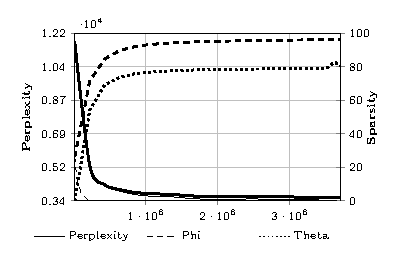
\includegraphics[width=70mm]{plot_perplexity_sparsity.eps}\\
    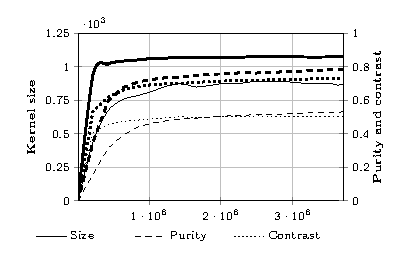
\includegraphics[width=70mm]{plot_kernel.eps}
\caption{Comparison of LDA (thin) and ARTM (bold) models. The number of processed documents is shown along the X~axis.}
\label{fig:comparison_plot}
\end{figure}

\paragraph{Text classification}

Support vector machine (SVM) based on token frequencies is known to be one of the best methods for text classification.
However, according to \cite{rubin12statistical} topic models demonstrate even better quality in case of unbalanced interdependent and intersecting classes.
Our experiment aims to prove that multimodal regularized topic models in BigARTM are as good as Dependency~LDA from~\cite{rubin12statistical}.
Dependency~LDA is in fact a~multimodal topic model with two modalities: words and class labels.

The EUR-lex collection contains about $20$K documents
split into train and test sets to provide the reproducibility of the results~\cite{rubin12statistical}.
The original size of the dictionary is over 190K~tokens.
Preprocessing from~\cite{rubin12statistical} removes all tokens encountered less than 20~times,
and reduces the dictionary to about $20$K tokens.
Class labels, encountered only once, are also removed to result in about 3250~classes.
Each document might belong to several classes.

For both Dependency LDA and ARTM the label regularization~\cite{rubin12statistical} was used.
The quality measures in our experiment are as follows:
AUC$_{PR}$~--- the area under the precision-recall curve;
AUC~--- the area under ROC-curve;
OneErr~--- the ratio of documents with the most probable label not from the correct set;
IsErr~--- the ratio of documents with not ideal classification.

The results are provided in Table~\ref{tab:classification}.
ARTM performs better than both Dependency LDA and SVM by the three measures out of four.
It is interesting to note that
while the number of topics increases up to 15\,000,
ARTM provides better classification quality,
while the optimal number of topics for Dependency LDA~is~200.

\begin{table}[t]
    \caption{Multimodal ARTM, Dependency LDA and SVM classification models.
        The best results are in bold. $T_{\mathrm{opt}}$ is the optimal number of topics.}
    \label{tab:classification}
    \medskip\centering\tabcolsep=5pt
    \begin{tabular}[t]{l|rrrrrr}
    \hline
     & $T_{\mathrm{opt}}$ & AUC$_{PR}\uparrow$ & AUC$\uparrow$ & OneErr$\downarrow$ & IsErr$\downarrow$ \\
    \hline
        ARTM  & 15\,000 & {\bf 0.529} & 0.980       & {\bf 27.1}  & {\bf 94.2}  \\
        DLDA  & 200   & 0.492       & {\bf 0.982} & 32.0        & 97.2        \\
        SVM   & --    & 0.435       & 0.975       & 31.6        & 98.1        \\
    \hline
    \end{tabular}
\end{table}

\paragraph{Cross-language search}
The following experiment shows that multimodal topic model may be used as multilingual one,
with languages of parallel texts treated as modalities.
The experiment was held on the \mbox{EuroParl} collection~\cite{koehn05parallel} of European Parliament Proceedings.
Proceedings in English and Spanish were chosen, as these languages are often used for multilingual topic model comparison.
As in \cite{mimno09polylingual,platt10translingual,mimno12sparse},
a~single document is a speech of one speaker at one session.

We use precision to measure quality of the cross-language search.
The precision is defined as the fraction of query documents~$q$ closest to their own translation $t$,
according to Hellinger distance:
\[
    H^2(d,q)= \frac12 \sum_{t\in T} \bigl( \sqrt{p(t\cond d)} - \sqrt{p(t\cond q)} \bigr)^2 .
\]
Training set includes proceedings from 1996 to 1999, and from 2001 to 2002,
test set includes proceedings of 2000 and the first 9 months of 2003.
The same partitioning is used in~\cite{platt10translingual} and~\cite{mimno12sparse}.
Moreover, as in \cite{mimno09polylingual,mimno12sparse},
the test comprised documents of the length more or equal than 100~words.
The total number of documents is~67379 in the training set, and 16068 in the test set.
Built-in capability of BigARTM to filter the dictionary was used:
all rare words, that appear in less than 20~documents, and stop-words, that appear in more than~50\% of documents, were discarded.
Table~\ref{tab:cross-lingual} shows the comparison of
models from \cite{mimno09polylingual,platt10translingual,mimno12sparse} and our ARTM.
For the first two models, the authors provide search precision for 50 topics only.
ARTM performs slightly worse than JPLSA, but we note, that
one iteration of BigARTM takes 30~seconds for 50~topics and 40~seconds for 100~topics,
while one iteration of JPLSA takes 31~minutes.
ARTM performs better if compared with models from \cite{mimno12sparse}.

\begin{table}[t]
\caption{Cross-language search precision for different models. The best value in each column is bolded.}
\label{tab:cross-lingual}
\medskip\centering\tabcolsep=4.3pt
\begin{tabular}{l|rrrr}
\hline
	& \multicolumn{4}{c}{Number of topics $T$} \\
\hline
Model &	50	&100	&200	&500 \\
\hline
PLTM \cite{mimno09polylingual}          &0.812  &  --  &  --  &  --  \\
JPLSA \cite{platt10translingual}        &\textbf{0.989}  &  --  &  --  &  --  \\
PLTM-He \cite{mimno12sparse}            &0.943  &0.985 &0.994 &0.993 \\
PLTM-He kd-trees \cite{mimno12sparse}	&0.949	&0.989 &0.995 &0.996 \\
\hline
BigARTM	                                &0.972	&\textbf{0.990} &\textbf{0.996} &\textbf{0.997} \\
\hline
\end{tabular}
\end{table}


%To~show how BigARTM works with multimodal datasets we prepared a text corpus
%containing all English and Russian Wikipedia articles with mutual interlanguage links.
%We represent each linked pair of articles
%as a single multi-language document with~two modalities, one modality for each language.
%That is how our multi-language collection acts as a multimodal document collection.
%
%The dump of Russian articles%
%\footnote{\url{http://dumps.wikimedia.org/ruwiki/20141203/}}
%had been processed following the same technique as we previously used in experiments on English Wikipedia.
%Russian words were lemmatized with Yandex MyStem~3.0%
%\footnote{\url{https://tech.yandex.ru/mystem/}}.
%To further reduce the dictionary we only keep words
%that appear in no less than 20~documents, but no~more than in~10\% of~documents in the collection.
%The resulting collection contains 216175~pairs of Russian--English articles, with combined dictionary
%of 196749 words (43\% Russian, 57\% English words).
%
%We build multi-language model with 400~topics.
%They cover a wide range of themes such as science, architecture, history, culture, technologies, army, different countries.
%%Most of them can be easily interpreted.
%All $400$ topics were reviewed by an independent assessor,
%and he successfully interpreted all except four topics.

%Table \ref{tab:top10words} shows top 10 words for four randomly selected topics.
%Top words in these topics are clearly consistent between Russian and English languages.
%The Russian part of last topic contains some English words such as
%``Windows'' or ``Server'' because it is common to use them in Russian texts without translation.

%\begin{table}[t!]
%	\caption{
%        Top 10 words with $p(w\cond t)$ probabilities (in~\%) from two-language topic model,
%        based on Russian and English Wikipedia articles with mutual interlanguage links.}
%	\label{tab:top10words}
%	\centering\tabcolsep=3pt%\small
%	\footnotesize
%    \begin{tabular}{|lr|lr||lr|lr|}	
%    	\hline
%    	\multicolumn{4}{|c||}{\textbf{Topic~68}} & \multicolumn{4}{c|}{\textbf{Topic~79}\rule{0pt}{3ex}} \\
%    	\hline
%    	research & 4.56 & институт & 6.03 & goals & 4.48 & матч & 6.02 \\
%    	technology & 3.14 & университет & 3.35 & league & 3.99 & игрок & 5.56 \\
%    	engineering & 2.63 & программа & 3.17 & club & 3.76 &  сборная & 4.51 \\
%    	institute & 2.37 & учебный & 2.75 & season & 3.49 & фк & 3.25 \\
%    	science & 1.97 & технический & 2.70 & scored & 2.72 & против & 3.20 \\
%    	program & 1.60 & технология & 2.30 & cup & 2.57 & клуб & 3.14 \\
%    	education & 1.44 & научный & 1.76 & goal & 2.48 & футболист & 2.67 \\
%    	campus & 1.43 & исследование & 1.67 & apps & 1.74 & гол & 2.65 \\
%    	management & 1.38 & наука & 1.64 & debut & 1.69 & забивать & 2.53 \\
%    	programs & 1.36 & образование & 1.47 & match & 1.67 & команда & 2.14 \\
%    	\hline
%    	\multicolumn{4}{|c||}{\textbf{Topic~88}} &     \multicolumn{4}{c|}{\textbf{Topic~251}\rule{0pt}{3ex}}  \\
%    	\hline
%        opera & 7.36 & опера & 7.82 & windows & 8.00 & windows & 6.05 \\
%    	conductor & 1.69 & оперный & 3.13 & microsoft & 4.03 & microsoft & 3.76 \\
%    	orchestra & 1.14 & дирижер & 2.82 & server & 2.93 & версия & 1.86 \\
%    	wagner & 0.97 & певец & 1.65 & software & 1.38 & приложение & 1.86 \\
%    	soprano & 0.78 & певица & 1.51 & user & 1.03 & сервер & 1.63 \\
%    	performance & 0.78 & театр & 1.14 & security & 0.92 & server & 1.54 \\
%    	mozart & 0.74 & партия & 1.05 & mitchell & 0.82 & программный & 1.08 \\
%    	sang & 0.70 & сопрано & 0.97 & oracle & 0.82 &  пользователь & 1.04 \\
%    	singing & 0.69 & вагнер & 0.90 & enterprise & 0.78 & обеспечение & 1.02 \\
%    	operas & 0.68 & оркестр & 0.82 & users & 0.78 & система & 0.96 \\
%    	\hline
%	\end{tabular}
%\end{table}

\paragraph{Recommending articles of collective blog}

Here we describe how multimodal topic modeling can be used for recommending articles in a collective blog.
Collective blog is an on-line platform where users can publish articles and respond to the articles of other authors.
To~make recommendations we add user's positive feedback to the article as a  modality.
For the experiment we used dataset of about $130$K articles with user feedback from \url{http://habrahabr.ru}~---
the most popular IT-oriented social blogging platform in Russia.
The articles from our dataset have five modalities:
words from text, users who liked articles, authors, tags and categories (hubs) specified by users.

To construct list of recommended articles to the user~$u$
we estimate his topic distribution $p(t\cond u)$ and rank documents according to $p(d\cond u)$.
To assess the quality of recommendations
we split the set of user--article interactions (likes) on two disjoint subsets in proportion $1:1$,
the former subset is used for estimating user topics and
the latter subset contains hold-out preferences used to compute Recall@$k$ metric
(the proportion of liked articles among top $k$ recommendations).
As a baseline recommendation model we used weighted regularized matrix factorization~\cite{hu08ials} based on user likes.
This approach is commonly used in recommender systems.

\begin{table}[t]
	\caption{
    The quality of recommendations for baseline matrix factorization model,
    unimodal model with only modality of user likes, and
    two multimodal models incorporating words and user-specified data (tags and categories).
	}
	\label{tab:habrahabr_recommendation_comparison}
    \centering\tabcolsep=4.3pt
	\begin{tabular}[t]{c|c|c|c}
	\hline
	Model & Recall@5 & Recall@10 & Recall@20 \\
	\hline
	baseline~\cite{hu08ials} & 0.591 & 0.652 & 0.678 \\
	likes & 0.62 & 0.59 & 0.65 \\
	likes + words & 0.79 & 0.64 & 0.68 \\
	all modalities & \bfseries{0.80} & \bfseries{0.71} & \bfseries{0.69} \\
	no regularization & 0.79 & 0.71 & 0.68 \\
	\hline
	\end{tabular}
\end{table}

Table \ref{tab:habrahabr_recommendation_comparison} presents the results of a comparison of three models.
Performance of the topic models is comparable or better than baseline.
Additional modalities improves recommendation ranking significantly.
The combination of all modalities with regularizers of sparsity and decorrelation
does not degrade the quality of recommendation but provides much more sparse and interpretable model.
%Another advantage of multimodal topic model over convenient matrix factorization techniques is an interpretability of factors.
It~is~well known that factors of Weighted Matrix Factorization are dense and their components do not correspond to human-sensible topics.
By~using regularizers we could make interpretability of factors even better.
The interpretability of the user profile $p(t\cond u)$ enables new ways of using recommendation model.

%Table \ref{tab:habrahabr_recommendation_comparison} presents the results of a comparison of three models.
%They show that a hybrid (multi-modal) model outperforms the unimodal model.
%Table~6 shows an example of the recommendations for randomly selected user $X$ in comparison with a list of articles that he commented.

%Regularization coefficients: Theta_sparsity=-0.2, phi_sparsity(words)=-0.2, phi_sparsity(authors)=-0.1, phi_sparsity(commentators)=-0.2, phi_sparsity(tags)=-0.2, phi_sparsity(hubs)=-0.1, decorrelation=10000000
%
%Grid search:
%decorrelation from 100 to 10000000
%Phi and Theta sparsity - from -1.0 to 1.0 step 0.1


\section{Conclusions}
\label{sec:Conclusions}
We have presented an Additive Regularization of Topic Models (ARTM),
a~powerful non-Bayesian framework for topic model inference.
ARTM facilitates the development of topic models and allows merging models together in arbitrary combinations.
Combining multiple modalities with multiple regularization criteria
covers dozens of models previously studied only in the Bayesian settings.

\mbox{BigARTM} is an open source project
for parallel online multimodal regularized topic modeling of large text collections.
Its~implementation is faster than existing popular topic modeling tools.
\mbox{BigARTM} provides high flexibility for various applications due to
multimodality and additive combinations of regularizers.
\mbox{BigARTM} has a built-in library of regularizers and quality measures.

\mbox{BigARTM} architecture has a~rich potential.
In future version it will be extended to run on a~distributed cluster environment,
improve performance and reduce memory usage for sparse topic models,
implement APIs for Java and C\#.

\bigskip
\subsubsection*{Acknowledgements.}
\nopagebreak
The work was supported by~the Russian Foundation for Basic Research (14-07-00847, 14-07-00908, 14-07-31176)
and by~Skolkovo Institute of Science and Technology (081-R).


%%%%%%%%%%%%%%%%%%%%%%%%%%%%%%%%%%%%%%%%%%%%%%%%%%%%%%%%%%%%%%%%%%%%%%%%%%%%
%\bibliographystyle{abbrv}
%\bibliography{MachLearn}
%%%%%%%%%%%%%%%%%%%%%%%%%%%%%%%%%%%%%%%%%%%%%%%%%%%%%%%%%%%%%%%%%%%%%%%%%%%%
%\pagebreak
\begin{thebibliography}{10}
\nopagebreak
\bibitem{bassiou14online}
N.~Bassiou and C.~Kotropoulos.
\newblock Online PLSA: Batch updating techniques including out-of-vocabulary words.
\newblock {\em Neural Networks and Learning Systems, IEEE Transactions on},
  25(11):1953--1966, Nov 2014.

\bibitem{blei12ptm}
D.~M. Blei.
\newblock Probabilistic topic models.
\newblock {\em Communications of the ACM}, 55(4):77--84, 2012.

\bibitem{blei03modeling}
D.~M. Blei and M.~I. Jordan.
\newblock Modeling annotated data.
\newblock In {\em Proceedings of the 26th Annual International ACM SIGIR
  Conference on Research and Development in Informaion Retrieval}, pages
  127--134, New York, NY, USA, 2003.

\bibitem{blei03latent}
D.~M. Blei, A.~Y. Ng, and M.~I. Jordan.
\newblock Latent {Dirichlet} allocation.
\newblock {\em Journal of Machine Learning Research}, 3:993--1022, 2003.

\bibitem{chien13bayesian}
J.-T. Chien and Y.-L. Chang.
\newblock Bayesian sparse topic model.
\newblock {\em Journal of Signal Processessing Systems}, 74:375--389, 2013.

\bibitem{cohn00missing}
D.~A. Cohn and T.~Hofmann.
\newblock The missing link~--- a~probabilistic model of document content and
  hypertext connectivity.
\newblock In {\em NIPS}, pages 430--436, 2000.

\bibitem{daud10knowledge}
A.~Daud, J.~Li, L.~Zhou, and F.~Muhammad.
\newblock Knowledge discovery through directed probabilistic topic models: a~survey.
\newblock {\em Frontiers of Computer Science in China}, 4(2):280--301, 2010.

\bibitem{smet09weblinking}
W.~De~Smet and M.-F. Moens.
\newblock Cross-language linking of news stories on the web using interlingual topic modelling.
\newblock In {\em Proceedings of the 2Nd ACM Workshop on Social Web Search and Mining},
SWSM '09, pages 57--64, New York, NY, USA, 2009.

\bibitem{dietz07unsupervised}
L.~Dietz, S.~Bickel, and T.~Scheffer.
\newblock Unsupervised prediction of citation influences.
\newblock In {\em Proceedings of the 24th international conference on Machine learning}, ICML '07,
pages 233--240, New York, NY, USA, 2007.

\bibitem{eisenstein11sparse}
J.~Eisenstein, A.~Ahmed, and E.~P. Xing.
\newblock Sparse additive generative models of text.
\newblock In {\em ICML'11}, pages 1041--1048, 2011.

\bibitem{hoffman10online}
M.~D. Hoffman, D.~M. Blei, and F.~R. Bach.
\newblock Online learning for latent dirichlet allocation.
\newblock In {\em NIPS}, pages 856--864. Curran Associates, Inc., 2010.

\bibitem{hofmann99plsi}
T.~Hofmann.
\newblock Probabilistic latent semantic indexing.
\newblock In~{\em Proceedings of the 22nd annual international ACM SIGIR
  conference on Research and development in information retrieval},
  pages 50--57, 1999.

\bibitem{hu08ials}
Y.~Hu, Y.~Koren and C.~Volinsky.
\newblock Collaborative filtering for implicit feedback datasets.
\newblock In {\em IEEE ICDM'08}. 2008.

\bibitem{khalifa13multi}
O.~Khalifa, D.~Corne, M.~Chantler, and F.~Halley.
\newblock Multi-objective topic modelling.
\newblock In {\em 7th International Conference Evolutionary Multi-Criterion
  Optimization (EMO 2013)}, pages 51--65. Springer LNCS, 2013.

\bibitem{koehn05parallel}
P.~Koehn.
Europarl: A Parallel Corpus for Statistical Machine Translation.
In {\em Conference Proceedings: the tenth Machine Translation Summit},
pages 79-86, Phuket, Thailand, 2005.

\bibitem{ugander11concave}
M.~O. Larsson and J.~Ugander.
\newblock A concave regularization technique for sparse mixture models.
\newblock In~{\em Advances in Neural Information Processing Systems 24}, pages 1890--1898, 2011.

\bibitem{liu11plda}
Z.~Liu, Y.~Zhang, E.~Y. Chang, and M.~Sun.
\newblock {PLDA+:} parallel latent {D}irichlet allocation with data placement and pipeline processing.
\newblock {\em ACM Trans. Intell. Syst. Technol.}, 2(3):26:1--26:18, May 2011.

\bibitem{mimno12sparse}
D.~Mimno, M.~Hoffman, and D.~Blei.
\newblock Sparse stochastic inference for latent Dirichlet allocation.
\newblock In J.~Langford and J.~Pineau, editors, {\em Proceedings of the 29th
  International Conference on Machine Learning (ICML-12)}, pages 1599--1606, 2012.

\bibitem{mimno09polylingual}
D.~Mimno, H.~M. Wallach, J.~Naradowsky, D.~A. Smith, and A.~McCallum.
\newblock Polylingual topic models.
\newblock In {\em Proceedings of the 2009 Conference on Empirical Methods in
  Natural Language Processing: Volume~2}, EMNLP '09, pages 880--889, 2009.

\bibitem{newman09distributed}
D.~Newman, A.~Asuncion, P.~Smyth, and M.~Welling.
\newblock Distributed algorithms for topic models.
\newblock {\em J. Mach. Learn. Res.}, 10:1801--1828, Dec. 2009.

\bibitem{newman06entity}
D.~Newman, C.~Chemudugunta, and P.~Smyth.
\newblock Statistical entity-topic models.
\newblock In {\em Proceedings of the 12th ACM SIGKDD International Conference
  on Knowledge Discovery and Data Mining}, KDD '06, pages 680--686, New York,
  NY, USA, 2006.

\bibitem{ni09mining}
X.~Ni, J.-T. Sun, J.~Hu, and Z.~Chen.
\newblock Mining multilingual topics from wikipedia.
\newblock In {\em Proceedings of the 18th International Conference on World Wide Web}, WWW '09,
pages 1155--1156, 2009.

\bibitem{platt10translingual}
J.~C.~Platt, K.~Toutanova, W.-T.~Yih.
\newblock Translingual document representations from discriminative projections.
\newblock In {\em Proceedings of the 2010 Conference on Empirical Methods in Natural Language Processing},
pages 251--261, Stroudsburg, PA, USA, 2010.

\bibitem{rehurek10software}
R.~\v{R}eh\r{u}\v{r}ek and P.~Sojka.
\newblock Software framework for topic modelling with large corpora.
\newblock In {\em Proceedings of the {LREC} 2010 Workshop on New Challenges for
  {NLP} Frameworks}, pages 45--50, Valletta, Malta, May 2010.

\bibitem{rubin12statistical}
T.~N. Rubin, A.~Chambers, P.~Smyth, and M.~Steyvers.
\newblock Statistical topic models for multi-label document classification.
\newblock {\em Machine Learning}, 88(1-2), pages 157--208, 2012.

\bibitem{shashanka07sparse}
M.~Shashanka, B.~Raj, and P.~Smaragdis.
\newblock Sparse overcomplete latent variable decomposition of counts data.
\newblock In J.~C. Platt, D.~Koller, Y.~Singer, and S.~Roweis, editors, {\em
  Advances in Neural Information Processing Systems, NIPS-2007}, pages
  1313--1320. MIT Press, Cambridge, MA, 2008.

\bibitem{si09taglda}
X.~Si and M.~Sun.
\newblock Tag-lda for scalable real-time tag recommendation.
\newblock {\em Journal of Information \& Computational Science}, 6:23--31,
  2009.

\bibitem{smola10architecture}
A.~Smola and S.~Narayanamurthy.
\newblock An architecture for parallel topic models.
\newblock {\em Proc. VLDB Endow.}, 3(1-2):703--710, Sept. 2010.

\bibitem{teh06hierarchical}
Y.~W. Teh, M.~I. Jordan, M.~J. Beal, D.~M. Blei.
\newblock Hierarchical {D}irichlet processes.
\newblock {\em Journal of the American Statistical Association}, {101}(476):1566--1581, 2006.

\bibitem{tihonov77methods-eng}
A.~N.~Tikhonov, V.~Y. Arsenin.
\newblock Solution of ill-posed problems.
\newblock W.~H. Winston, Washington, DC. 1977.

\bibitem{voron14dan-eng}
K.~V. Vorontsov.
\newblock Additive regularization for topic models of text collections.
\newblock {\em Doklady Mathematics}, 89(3):301--304, 2014.

\bibitem{voron14mlj}
K.~V. Vorontsov and A.~A. Potapenko.
\newblock Additive regularization of topic models.
\newblock {\em Machine Learning, Special Issue on Data Analysis and Intelligent Optimization}, 2014.

\bibitem{voron14aist}
K.~V. Vorontsov and A.~A. Potapenko.
\newblock Tutorial on probabilistic topic modeling: Additive regularization for stochastic matrix factorization.
\newblock In~{\em AIST'2014, Analysis of Images, Social networks and Texts},
  volume 436, pages 29--46. Springer International Publishing Switzerland,
  Communications in Computer and Information Science (CCIS), 2014.

\bibitem{voron15slds}
K.~V.~Vorontsov, A.~A.~Potapenko, and A.~V.~Plavin.
\newblock Additive Regularization of Topic Models for Topic Selection and Sparse Factorization.
\newblock In~{\em 3rd Int'l Symposium On Learning And Data Sciences (SLDS 2015)},
    Royal Holloway, University of London, UK.
    Springer, LNAI~9047, pages 193--202, 2015.

\bibitem{wang09decoupling}
C.~Wang and D.~M. Blei.
\newblock Decoupling sparsity and smoothness in the discrete hierarchical Dirichlet process.
\newblock In {\em NIPS}, pages 1982--1989. Curran Associates, Inc., 2009.

\bibitem{wang09plda}
Y.~Wang, H.~Bai, M.~Stanton, W.-Y. Chen, and E.~Y. Chang.
\newblock {PLDA}: Parallel latent {D}irichlet allocation for large-scale applications.
\newblock In {\em Proceedings of the 5th International Conference on
  Algorithmic Aspects in Information and Management}, pages 301--314, 2009.

\end{thebibliography}
%%%%%%%%%%%%%%%%%%%%%%%%%%%%%%%%%%%%%%%%%%%%%%%%%%%%%%%%%%%%%%%%%%%%%%%%%%%%

%\newpage
\section*{Appendix}

Consider the system of equations \eqref{eq:Estep}--\eqref{eq:Mstep:theta}.

A topic~$t$ is called \emph{regular} for a modality~$m$
if $n_{wt} + \phi_{wt} \frac{\partial R}{\partial \phi_{wt}} > 0$
for at least one term ${w\in W^m}$.
If~the~reverse inequality holds for all ${w\in W^m}$ then
the topic~$t$ is called \emph{irregular};
in this case the $t$-th vector-column in the matrix~$\Phi^m$ equals zero
and can not represent a~discrete distribution.
This means that the topic~$t$ for the modality~$m$ must be excluded from the model.
This mechanism can be used determine the optimal number of topics.

A document~$d$ is called \emph{regular}
if $n_{td} + \theta_{td} \frac{\partial R}{\partial \theta_{td}} > 0$
for at least one topic ${t\in T}$.
If~the reverse inequality holds for all ${t\in T}$ then
the document~$d$ is called \emph{irregular};
in this case the $d$-th vector-column in the matrix~$\Theta$ equals zero
and can not represent a~discrete distribution.
This means that the document~$d$ must be excluded from the model.
For example, it may be too short or irrelevant for the collection.

\begin{theorem}
\label{th:multimodal}
    If the function $R(\Phi,\Theta)$ is continuously differentiable
    and $(\Phi,\Theta)$ is the local maximum
    of the problem~\eqref{eq:multimodal},~\eqref{eq:multimodal:norm}
    then for any regular topic~$t$ and any regular document~$d$
    the system of equations \eqref{eq:Estep}--\eqref{eq:Mstep:theta} holds.
\end{theorem}

\begin{proof}
    For the local minimum $\Phi^m,\Theta$
    of the problem~\eqref{eq:multimodal},~\eqref{eq:multimodal:norm}
    the Karush--Kuhn--Tucker (KKT) conditions can be written as follows:
    %(conditions with respect to $\theta_{td}$ are analogous):
    \begin{gather*}
        \sum_{d} n_{dw} \frac{\theta_{td}}{p(w\cond d)} + \frac{\partial R}{\partial \phi_{wt}}
        = \lambda_t - \lambda_{wt};
    \\
        \lambda_{wt}\geq 0;
        \quad
        \lambda_{wt}\phi_{wt} = 0;
    \\
        \sum_{m} \tau_m \!\!\sum_{w\in W^m}\!\! n_{dw} \frac{\phi_{wt}}{p(w\cond d)} + \frac{\partial R}{\partial \theta_{td}}
        = \mu_d - \mu_{td};
    \\
        \mu_{td}\geq 0;
        \quad
        \mu_{td}\theta_{td} = 0;
    \end{gather*}
    where $\lambda_t$, $\lambda_{wt}$, $\mu_d$, $\mu_{td}$
    are KKT multipliers for normalization and nonnegativity constraints.

    Let us multiply
    both sides of the first equation by~$\phi_{wt}$,
    both sides of the second equation by~$\theta_{td}$,
    and reveal the auxiliary variable~$p_{tdw}$ from~\eqref{eq:Estep}
    in~the~left-hand side of both equations.
    Then we sum
    the right-hand side of the first equation over~$d$,
    the right-hand side of the second equation over~$t$:
    \begin{gather*}
        \phi_{wt} \lambda_t
        =
        \sum_{d}
        n_{dw} \frac{\phi_{wt}\theta_{td}}{p(w\cond d)}
        + \phi_{wt} \frac{\partial R}{\partial \phi_{wt}}
        =
        n_{wt} + \phi_{wt} \frac{\partial R}{\partial \phi_{wt}};
    \\
        \theta_{td} \mu_{d}
        =
        \sum_{m} \tau_m \!\!\!\sum_{w\in W^m}\!\!\!
        n_{dw} \frac{\phi_{wt}\theta_{td}}{p(w\cond d)}
        + \theta_{td} \frac{\partial R}{\partial \theta_{td}}
        =
        n_{td} + \theta_{td} \frac{\partial R}{\partial \theta_{td}}.
    \end{gather*}

    An~assumption that $\lambda_t\leq 0$ contradicts the regularity condition for the $(t,m)$ pair.
    Then ${\lambda_t>0}$.
    Either ${\phi_{wt}= 0}$ or both sides of the first equation are positive.
    Combining these two cases in one formula, we write:
    \begin{equation}
    \label{eq:in-theorem-1:phi}
        \phi_{wt} \lambda_t
        =
        \max\biggl\{
        n_{wt} + \phi_{wt} \frac{\partial R}{\partial \phi_{wt}}, 0
        \biggr\}.
    \end{equation}
    Analogously,
    an~assumption that $\mu_d\leq 0$ contradicts the regularity condition for the document~$d$.
    Then ${\mu_d>0}$.
    Either ${\theta_{td}= 0}$ or both sides of the second equation are positive,
    consequently,
    \begin{equation}
    \label{eq:in-theorem-1:theta}
        \theta_{td} \mu_d
        =
        \max\biggl\{
        n_{td} + \theta_{td} \frac{\partial R}{\partial \theta_{td}}, 0
        \biggr\}.
    \end{equation}

    Let us sum
    both sides of~the first equation over all~${w\in W^m}$,
    then
    both sides of~the second equation over all~${t\in T}$:
    \begin{gather}
    \label{eq:in-theorem-2:phi}
        \lambda_t
        =
        \sum_{w\in W^m}
        \max\biggl\{
        n_{wt} + \phi_{wt} \frac{\partial R}{\partial \phi_{wt}}, 0
        \biggr\};
    \\
    \label{eq:in-theorem-2:theta}
        \mu_d
        =
        \sum_{t\in T}
        \max\biggl\{
        n_{td} + \theta_{td} \frac{\partial R}{\partial \theta_{td}}, 0
        \biggr\}.
    \end{gather}

    Finally,
    we obtain~\eqref{eq:Mstep:phi} and~\eqref{eq:Mstep:theta}
    by expressing $\phi_{wt}$ from~\eqref{eq:in-theorem-1:phi} and \eqref{eq:in-theorem-2:phi},
    then
    by expressing $\theta_{td}$ from~\eqref{eq:in-theorem-1:theta} and \eqref{eq:in-theorem-2:theta}.
    \qed
\end{proof}

\end{document}

